\section{Requirements}
\label{section:requirements}

The requirements for our software stem from the growing need for parallel
analysis in the domain of climate science\cite{MODSIM07:LOT} but also from
the use of the geodesic grid.

\subsection{Geodesic Grid}
\label{subsection:grid}

Until recently, climate and weather models have primarily been simulated on
structured grids that divide the latitude and longitude axes in even
increments, resulting in logically structured simulation grids. Standard
conventions for describing this data in the NetCDF data model have been
formalized by the Climate and Forecast (CF) conventions\cite{CF}. CF defines
conventions and metadata standards that enable both human and computer
interpretation of the data.  Human interpretation is supported through the use
of standard names while definition of spatial and temporal properties of the
data have enabled an extensive set of tools for data manipulation and display
such as \cite{NCO}, \cite{OPeNDAP}, and \cite{FERRET}.  The CF Conventions
have been evolving to support many variations of structured grids including
Orthographic, Polar stereographic, Transverse Mercator, and many others . 

The GCRM uses a geodesic grid.  The geodesic grid is created by recursively
bisecting an icosahedron of 20 triangular faces and twelve vertices and
projecting the resulting faces onto a unit sphere.  The resulting vertices
represent the centers of hexagonal grid cells with the exception of twelve
pentagons (the centers of the original twelve vertices.) See Figure
\ref{fig:geodesic} for an example of the first stage of bisection and
projection, followed by the definition of one of the hexagons.  Further
details can be found in \cite{GEODESIC}.

\begin{figure}[!t]
\center
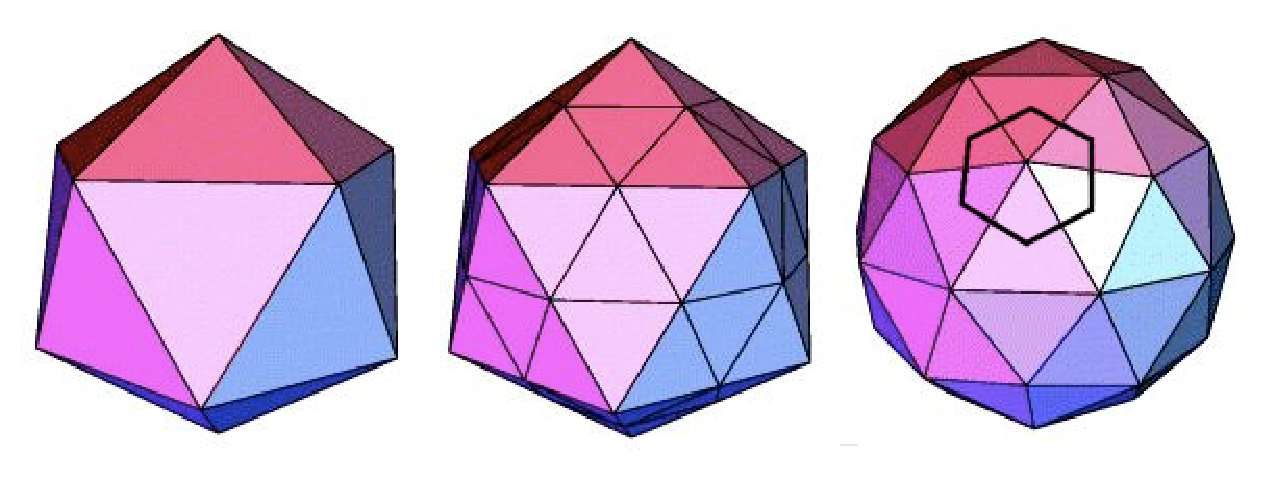
\includegraphics[width=3.5in]{images/geodesic2}
\caption{First stage generation of the geodesic grid}
\label{fig:geodesic}
\end{figure}

From the previous description, it can be seen that the geodesic grid used by
the GCRM is fairly regular. However, the horizontal dimension has some
important properties in common with unstructured grids: the grid coordinates
are not monotonic and simple conventions are not available for identifying the
neighbors of all cells.  As a consequence, it is necessary provide more
information about the topology of the grid. Other unstructured grids such as
triangular, cubed sphere \cite{CUBE}, and arbitrary unstructured polygons are
also being applied to various models.  There is a recognized need to extend
the CF conventions to unstructured grids so that general data analysis,
regridding, and display tools can be developed. As yet, no such standard
exists.  Balaji has cataloged a number of unstructured grids \cite{Balaji} and
proposes a tiling approach to describing grids.  The tiling approach supports
embedded and nested grids but has been slow to gain momentum, in part due to
its complexity.  In the ocean modeling community, workshops to discuss
standards have taken place \cite{UGRIDS}, however, these efforts are still in
the early stages of development and acceptance.   Lacking a standard,
development of general purpose tools has been slowed.  However some
preliminary tools and approaches have progressed by focusing on the in-memory
operations and abstracting the data loading from the processing \cite{UGRID}. 

Although the geodesic grid is fairly structured, we choose to represent it in
an unstructured way.  Each of the grid's cells, corners, and edges are
uniquely indexed from zero.  For a given positive integer $R$, there are $N =
10 \times 2^{2R} + 2$ cells, $C = (N-2) \times 2$ corners, and $E = (N-2)
\times 3$ edges.  Increasing the value of $R$ increases the resolution of the
model.  For example, a value of $R=10$ is approximately 8Km while $R=11$ is
approximately 4Km.  The cells, corners, and edges are represented as
dimensions within a NetCDF file.

The horizontal topology describes the connectivity relationships between
cells, nodes, and edges, all of which may have associated 3D data.  The
topology consists of three primary arrays: a mapping between cells and cell
corners, a mapping between cells and cell edges, and a mapping between edges
and corners.  Because neighbor lists are important for visualization programs
but difficult to generate in the general case, they are included as part of
the topology as the \verb+cell_neighbors(cells,neighbors=6)+ variable.  The
full list of topology variables include:

\begin{itemize}
\item \verb+cell_neighbors(cells,neighbors=6)+,
\item \verb+cell_corners(cells,cellcorners=6)+,
\item \verb+cell_edges(cells,celledges=6)+, and
\item \verb+edge_corners(edges,edgecorners=2)+
\end{itemize}

The vast majority of cells are hexagons which is why most of the last
dimensions are of size six except for the obvious case of \verb+edge_corners+.
For the twelve pentagons, the sixth value in these arrays are repeated but
could just have easily been set to a negative index and interpreted
appropriately.

The horizontal geometry describes the longitude and latitude location of each
object.  That is, there is one latitude and one longitude array for each of
the topology objects (cell centers, corners, and edges).

The vertical grid consists of layers sandwiched between interfaces with the
number of layers equal to the number of interfaces minus 1.   Because grid
variables are associated with both locations, layers and interfaces are
defined as dimensions.  They can be thought of as two distinct vertical grids
from a representation standpoint.

The data model is designed to support efficient model output, fully describe
the grid topology, and provide the sufficient information for tessellation to
triangles for 3D visualization.  The approach taken with the model is to adopt
the CF conventions to the extent possible and adopt early ideas circulating
within the community.  However, as many of the details have not been decided,
custom data analysis tools are currently required.

\subsection{Data Parallelism}

Larson, Ong, and Tokarz note that the current popular climate data analysis
packages remain single-processor applications which lack the memory required
to handle large data volumes as well as the processing power to analyse the
data in a timely fashion\cite{MODSIM07:LOT}.  Although they emphasize using
OpenMP as a first step toward parallism, we instead emphasize using a
distributed data model first.  Well designed communication libraries such as
the Message Passing Interface (MPI)\cite{MPI} may already take advantage of
shared-memory parallelism within a compute node or multi-core desktop
computer.

The data parallelism offered by libraries such as MPI or Global Arrays is
absolutely necessary to handle the size of data of modern climate models.  An
edge data variable of the geodesic grid at an approximate resolution of 4Km
and 100 levels is nearly $10 \times 2^{2R} \times 3 \times 100 \times 4
\unit{bytes} \approx 50 \unit{gigabytes}$ in size.  Even a modest number of
these variables will surpass the memory available in most desktop systems and
even some small clusters.

\subsection{Fast IO}

For data of this size, efficiently reading from and writing to disk requires
the use of parallel IO libraries such as Parallel NetCDF\cite{PNETCDF} or the
HDF5/NetCDF4\cite{HDF5}\cite{NETCDF}, both of which are in turn built on top
of the MPI-IO libraries\cite{MPIIO}.  Currently, GCRM output is stored in
netCDF\cite{NETCDF} files, a format for storing array-oriented
machine-independent data.

\subsection{Dataset Abstraction}

Model output is often distributed across many files for a given model run.
There are any number of schemes for organizing so many files e.g. one variable
per file with multiple timesteps per file, separating out the grid into a
separate file, one timestep per file with multiple variables.  The
reconstitution of these files into a logical set of variables and metadata is
an established practice\cite{NcML,THREDDS}.  We emphasize that the aggregation
of files into an abstract dataset is required in order to operate on the data
itself.  Operations on a dataset are more intuitive than needing to know the
addling details of which files hold which variables.

\subsection{Maintenance of Topology Variables}

Regular grids such as the cartesian, rectilinear, or curvilinear lend
themselves to representations as multidimensional arrays such that logically
adjacent cells are either adjacent in memory or can be located via a
shape-based index calculation.  Although some attempt is made to keep
logically adjacent cells nearby in memory, geodesic grids do not have the
luxury of using relatively simple shape-based index arithmetic to locate
neighbors.

The topology variables mentioned in \ref{subsection:grid} are not unique to
our grid; any grid could be described using a similar set of variables.
However, since topology is often implicitly defined by other grids, these
variables are not correctly handled by current software.  When a subset
occurs, the indices of these variables must be updated to reflect the
remaining corners, edges, and cells.

\subsection{Maintain Integrity of Entire Grid Cells}

Howe and Maier detail the properties of well-formed grids in \cite{UGRID}.
Proper subsets should maintain the same well-formed properties of the original
in order to remain useful to further analysis.  Therefore, the cell and its
surrounding corners and edges must remain intact during a subset.
